\chapter{Typical Use Cases}

\section{Transfer function and full result}

\subsection{SISO system}

The most common use case of \linnet{} is the computation of the frequency
response of a single in- and output system. This use case demonstrates how
such a basic investigation can be done with \linnet{}.

% Use case SISO: OP filter with two time constants.
{
% This define is related to the specifics of the array package; see
% http://texwelt.de/wissen/fragen/3401/zentrieren-text-in-tabelle (as of
% July 25 2014) for more
\newcolumntype{M}[1]{>{\centering\arraybackslash}m{#1}}

\begin{figure}
\begin{center}
\begin{tabular}{M{6cm}M{5.4cm}}
{\normalsize
\verbatiminput{UseCaseOpFilter.cnl}
}
&
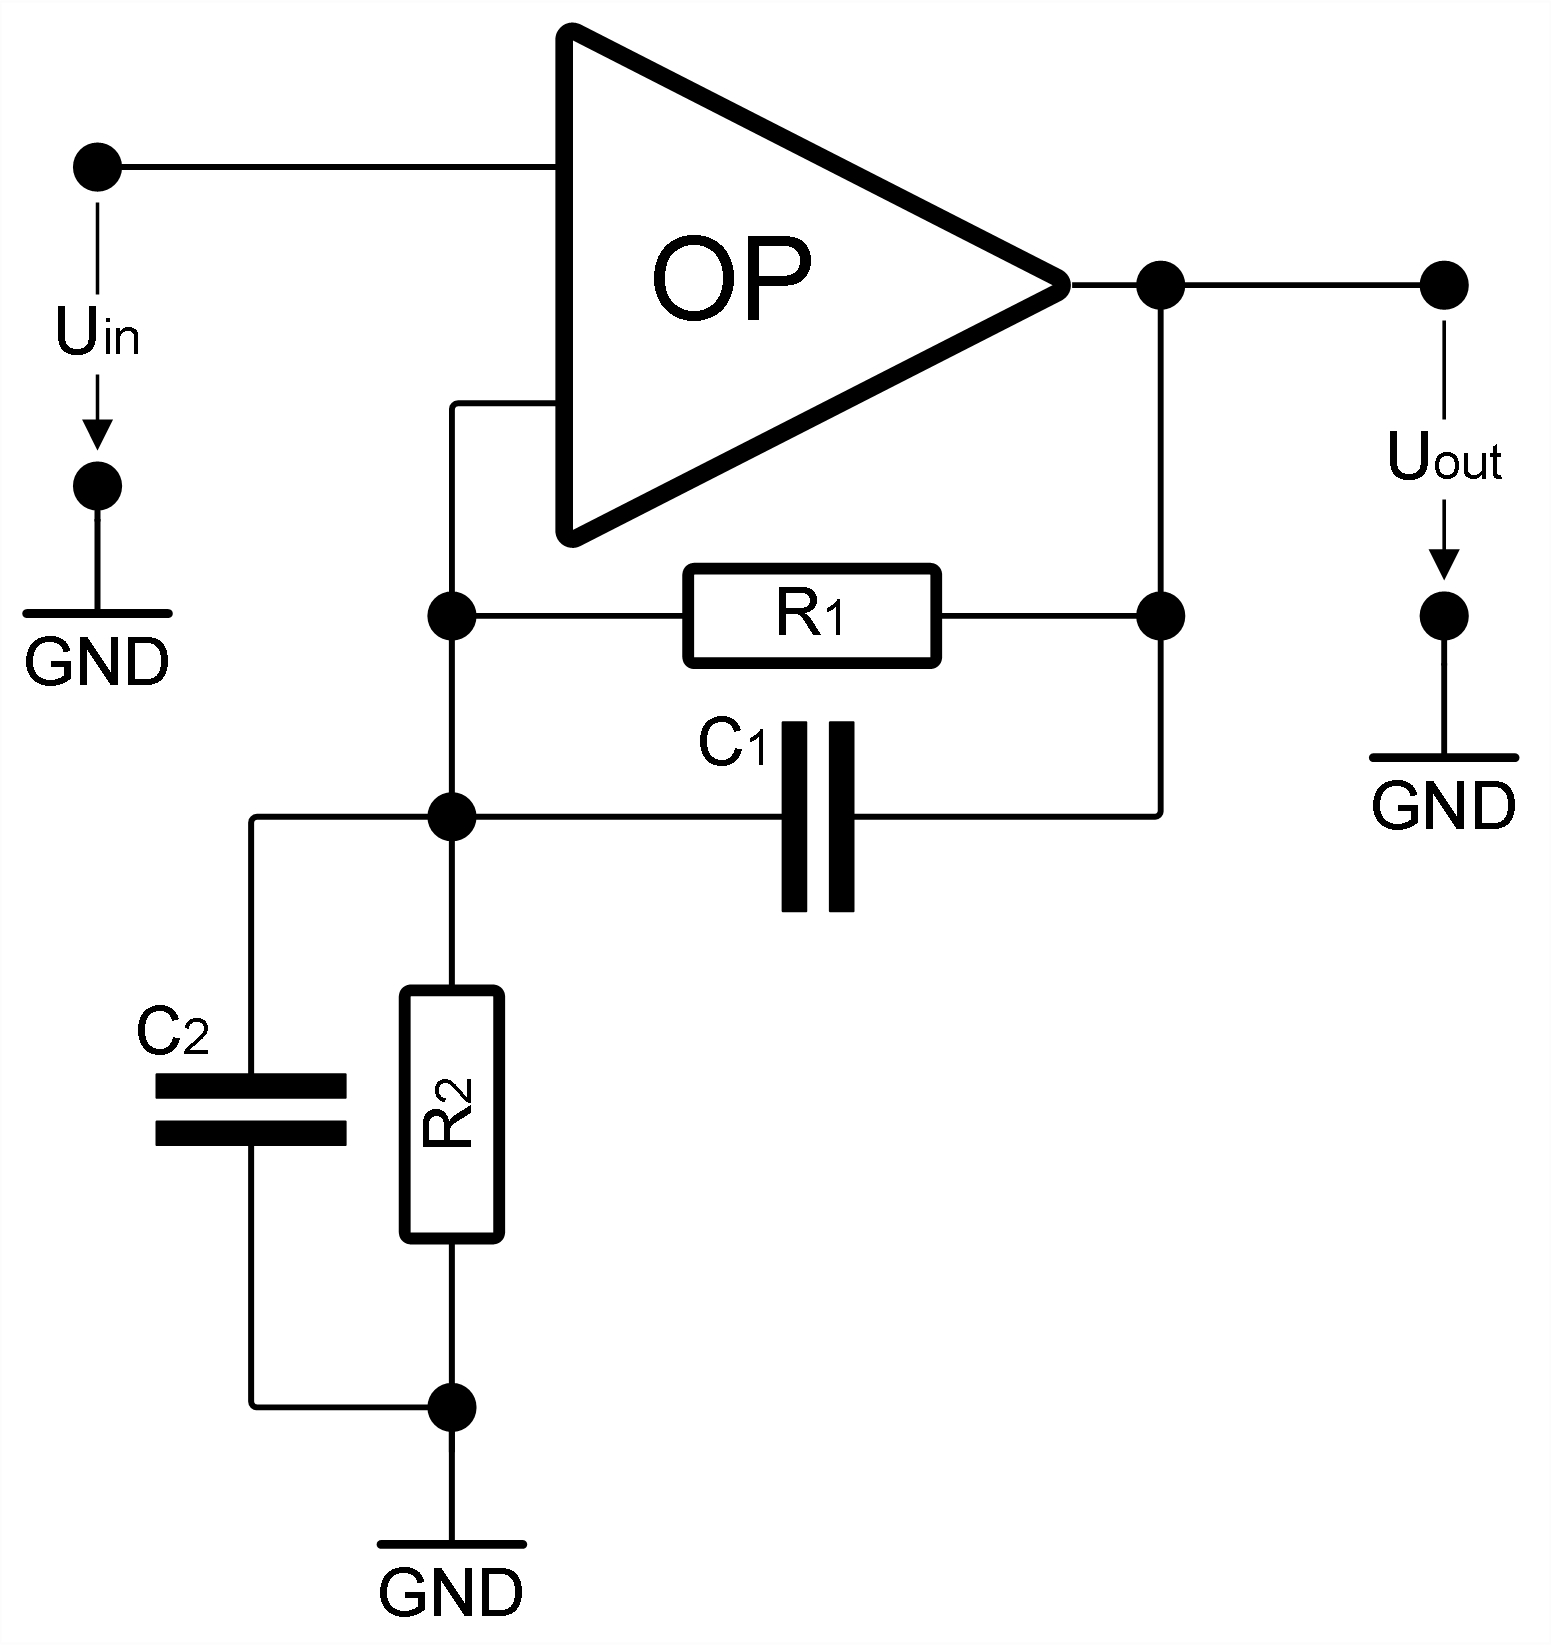
\includegraphics[width=5.4cm]{UseCaseOpFilter}
\\

\end{tabular}
\caption{Op-amp filter with two time constants}
\label{figUseCaseOpFilter}
\end{center}
\end{figure}
} % End of figure use case SISO: OP filter with two time constants.

Please refer to figure \ref{figUseCaseOpFilter}. The circuit implements a
typical op-amp based filter. It has two time constants; between the two
edge frequencies the amplification rises from its initial DC value to the
final value for high input frequencies. The device values are chosen such
that all relevant frequencies are in the audio frequency range and the
amplification increase is about 20\,dB.

The netlist, which is printed on the left hand side of the figure be
stored in the file \file{opFilter.cnl}. \linnet{} is run with the command
line
\begin{verbatim}
linnet -l -o opFilter.cnl
\end{verbatim}

The most natural thing to do is to compute the transfer function of the
filter, i.e. the dependency of the output signal on the input signal as a
complex function. The line \verb+PLOT G Uout Uin+ specifies this result.
\linnet{} responds with:
\begin{verbatim}
RESULT - User-defined result G (Bode plot):
The dependency of Uout on Uin:
  Uout(s) = N_Uout_Uin(s)/D_Uout_Uin(s) * Uin(s), with
    N_Uout_Uin(s) = (R1*R2*C1 + R1*R2*C2) * s
                    +(R1 + R2)
    D_Uout_Uin(s) = R1*R2*C1 * s
                    +R2
\end{verbatim}

The second requested result, \ident{Gf}, uses the keyword \code{RES} in
the specification. A full result is demanded. \linnet{} responds with:
\begin{verbatim}
RESULT - User-defined result Gf:
The solution for unknown Uout:
  Uout(s) = N_Uout_Uin(s)/D_Uout_Uin(s) * Uin(s), with
    N_Uout_Uin(s) = (R1*R2*C1 + R1*R2*C2) * s
                    +(R1 + R2)
    D_Uout_Uin(s) = R1*R2*C1 * s
                    +R2
\end{verbatim}

\begin{figure}
\begin{center}
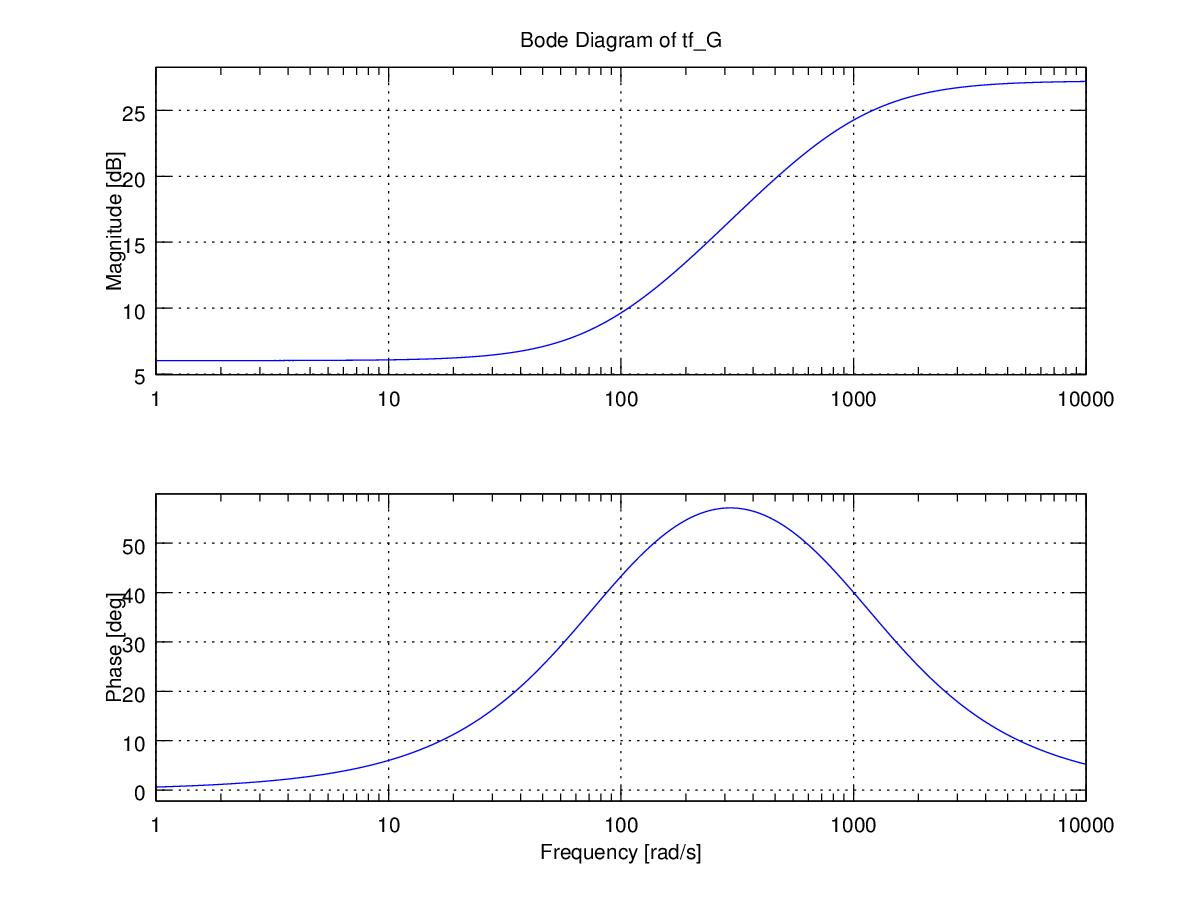
\includegraphics[width=12cm]{UseCaseOpFilter_Bode}
\caption{Default plot for \linnet{} result of kind \code{PLOT}}
\label{figUseCaseOpFilter_Bode}
\end{center}
\end{figure}

\begin{figure}
\begin{center}
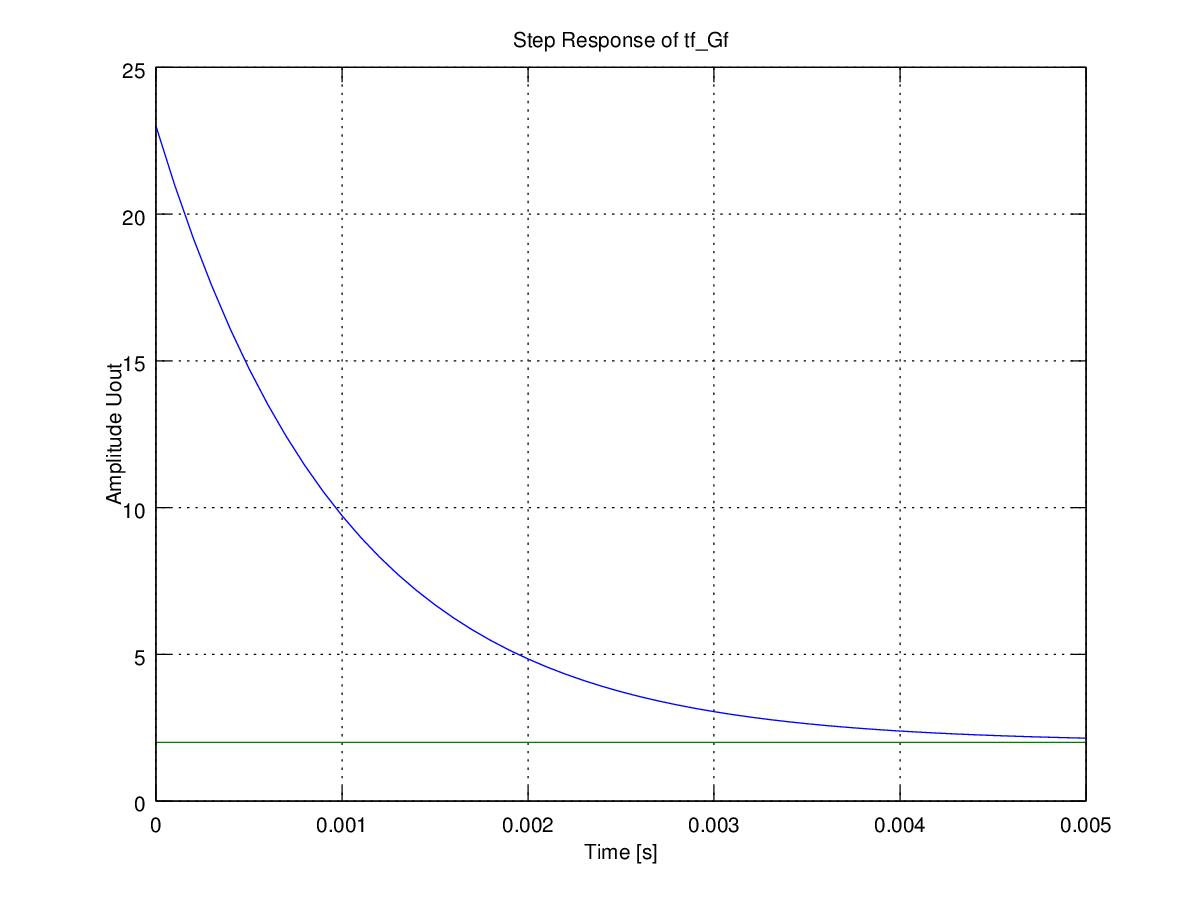
\includegraphics[width=12cm]{UseCaseOpFilter_step}
\caption{Default plot for \linnet{} result of kind \code{RES}}
\label{figUseCaseOpFilter_step}
\end{center}
\end{figure}

Actually, both results are just the same: The filter is a SISO system with
a single input and the full dependency of the output on this input is the
full dependency on \emph{all} inputs at the same time.

Only when looking at the generated Octave code one will recognize a
difference. While the generated LTI object is still identical differs the
default operation performed on this object in both cases. The results have
been implemented as Octave scripts \file{G.m} and \file{Gf.m} in the
output folder \file{opFilter}. If called just like that the default
operation is performed: The Octave command \code{G} opens a figure window
with a Bode plot (see figure \ref{figUseCaseOpFilter_Bode}), command
\code{Gf} presents the plot of the step response (see figure
\ref{figUseCaseOpFilter_step}). Regardless, both Octave scripts can be
applied to produce the same plots and numeric results if you make use of
the optional function parameters and return values. Please, refer to
section \ref{secOctaveInterface} for details.

The next result, which is specified in the netlist file is called
\ident{SIMO}. A full result is demanded for the three quantities
$U_{out}$, $U_{im}$ and $I_{op}$, where $U_{im}$ is the voltage at the
feedback input of the op-amp and $I_{op}$ its output current. \linnet{}
responds with:
\begin{verbatim}
RESULT - User-defined result SIMO:
The solution for unknown Uout:
  Uout(s) = N_Uout_Uin(s)/D_Uout_Uin(s) * Uin(s), with
    N_Uout_Uin(s) = (R1*R2*C1 + R1*R2*C2) * s
                    +(R1 + R2)
    D_Uout_Uin(s) = R1*R2*C1 * s
                    +R2
The solution for unknown U_Im:
  U_Im(s) = N_U_Im_Uin(s)/D_U_Im_Uin(s) * Uin(s), with
    N_U_Im_Uin(s) = 1
    D_U_Im_Uin(s) = 1
The solution for unknown I_OP:
  I_OP(s) = N_I_OP_Uin(s)/D_I_OP_Uin(s) * Uin(s), with
    N_I_OP_Uin(s) = R1*R2*C1*C2 * s^2
                    +(R1*C1 + R2*C2) * s
                    +1
    D_I_OP_Uin(s) = D_Uout_Uin(s)
\end{verbatim}

Again, the found formula for $U_{out}$ is exactly the same. However, this
time it's only one formula out of three, which make up the complete
result. For analytic considerations this is irrelevant. It doesn't matter
if one specifies three single results with \code{RES} or one result with
three dependent quantities. The only important difference can be found in
the generated Octave script: A true SIMO LTI object is created. If typing
\code{tf\_SIMO=SIMO} on the Octave command line all three partial transfer
functions of the SIMO system are printed.

The transfer function $I_{op}(U_{in})$ has a numerator degree in $s$ of
two but a denominator degree of only one, which means that the step
response of the output current has a Dirac impulse; the two capacitors
need to be loaded instantly. Octave can create such an LTI object, see
before, but can't plot the unreal step response; it complains about an
``improper'' system.

The direct capacitive connection of the op-amp's output to ground further
means an infinite output current for high frequencies. This is shown by
the Bode plot Octave presents when typing \code{Iop}, which is the name of
the last user-specified result. The Bode plot of an ``improper'' system
is possible, as long as it is a SISO system. (Octave refuses to draw Bode
plots of SIMO or MIMO systems.)


\subsection{MIMO system}

\linnet{} is not restricted to SISO systems. If more than one independent
sources are in the circuit then we have a multiple input system. \linnet{}
offers to compute all voltages and currents of a circuit, which leads to a
multiple output system. The following use case presents a typical MIMO
scenario.

% Use case MIMO: Analog add
{
% This define is related to the specifics of the array package; see
% http://texwelt.de/wissen/fragen/3401/zentrieren-text-in-tabelle (as of
% July 25 2014) for more
\newcolumntype{M}[1]{>{\centering\arraybackslash}m{#1}}

\begin{figure}
\begin{center}
\begin{tabular}{M{5.5cm}M{6.57cm}}
{\normalsize
\verbatiminput{UseCaseAnalogAdd.cnl}
}
&
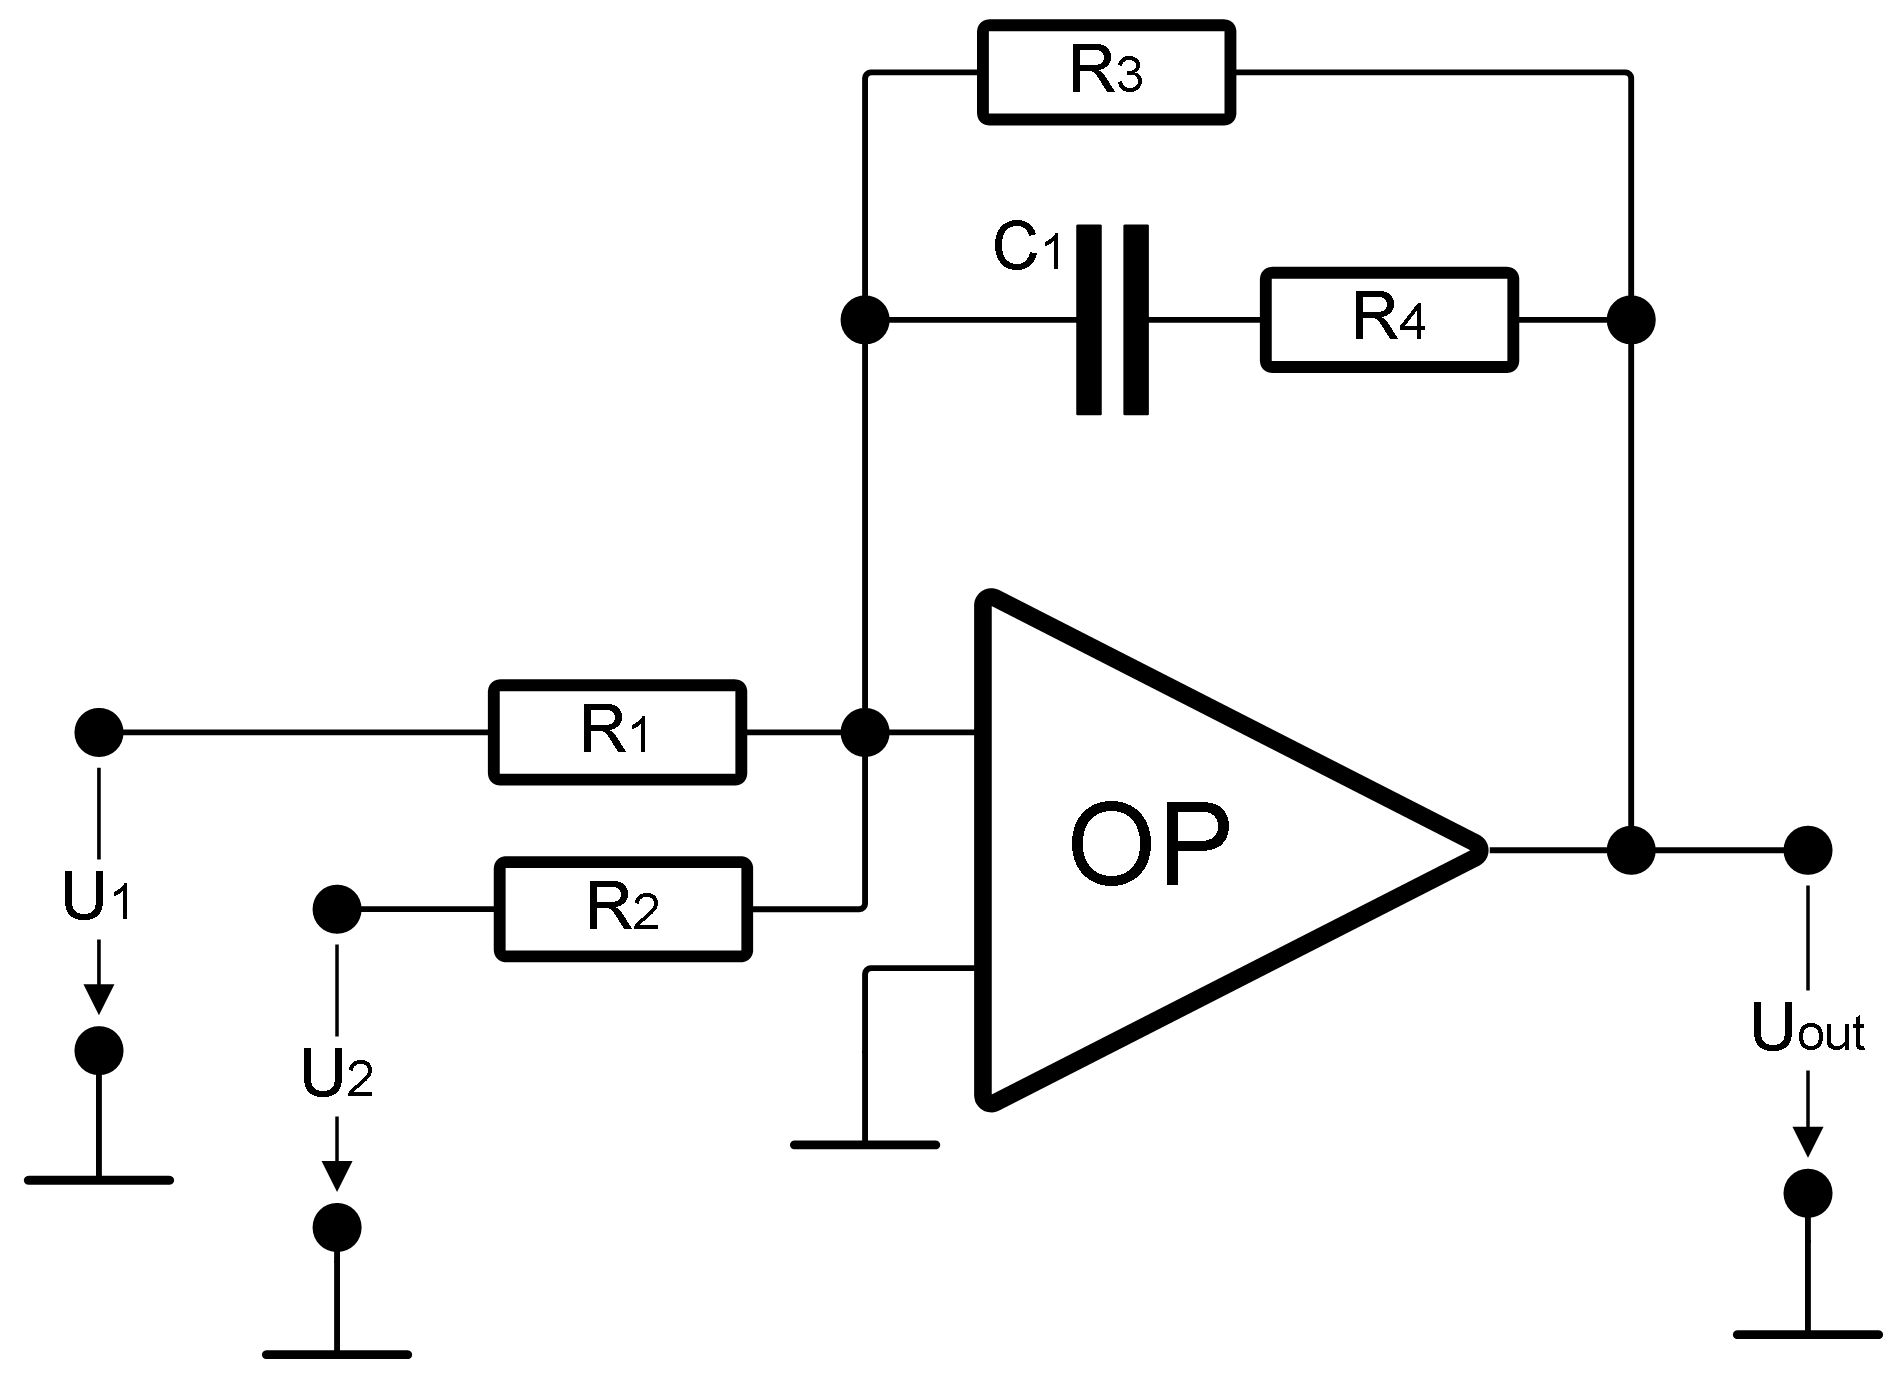
\includegraphics[width=6.57cm]{UseCaseAnalogAdd}
\\

\end{tabular}
\caption{MIMO example: Analog adder}
\label{figUseCaseAnalogAdd}
\end{center}
\end{figure}
} % End of figure for use case MIMO: Analog add

Figure \ref{figUseCaseAnalogAdd} shows an analog adder. The two input
signals are added in a weighted sum in the ratio 1:2. The result
specification \verb+RES MIMO U_out I_OP+ demands two dependents, this
means a MIMO system with two in- and two output. \linnet{} responds with:
\begin{verbatim}
RESULT - User-defined result MIMO:
The solution for unknown U_out:
  U_out(s) = N_U_out_U1(s)/D_U_out_U1(s) * U1(s)
             + N_U_out_U2(s)/D_U_out_U2(s) * U2(s), with
    N_U_out_U1(s) = -4*R1*C1 * s
                    -40
    D_U_out_U1(s) = 41*R1*C1 * s
                    +10
    N_U_out_U2(s) = -8*R1*C1 * s
                    -80
    D_U_out_U2(s) = D_U_out_U1(s)
The solution for unknown I_OP:
  I_OP(s) = N_I_OP_U1(s)/D_I_OP_U1(s) * U1(s)
            + N_I_OP_U2(s)/D_I_OP_U2(s) * U2(s), with
    N_I_OP_U1(s) = -1
    D_I_OP_U1(s) = R1
    N_I_OP_U2(s) = -2
    D_I_OP_U2(s) = R1
\end{verbatim}

The composition of a single result from multiple formulas is already known
from the previous use case, which introduced a SIMO system. Here, the
representation of the multiple inputs is new. Each output is represented
as a sum of two transfer functions, one for each input.

\begin{figure}
\begin{center}
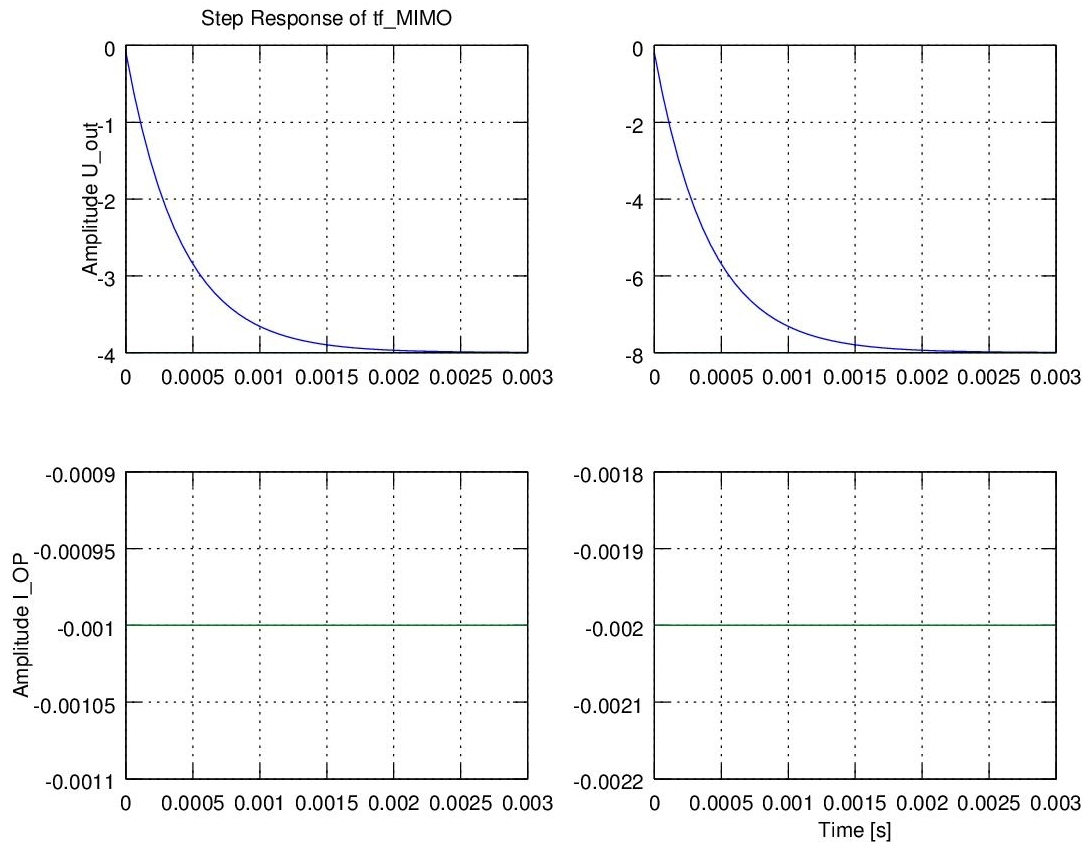
\includegraphics[width=8cm]{UseCaseAnalogAdd_step}
\caption{Step response of MIMO system created with \code{RES}}
\label{figUseCaseAnalogAdd_step}
\end{center}
\end{figure}

The generated Octave script \file{MIMO.m} will plot the step response of
the system, see figure \ref{figUseCaseAnalogAdd_step}. The step response is
presented in a rectangular grid for each in- and output. The meaning of a
single figure is the response of the related output if the related input
undergoes a step and all other inputs are constantly null.

The second user-specified result uses the keyword \code{PLOT}. The
dependency of a single quantity on a single other one is presented as Bode
plot. The result specification \verb+PLOT G1 U_out U1+ yields:
\begin{verbatim}
RESULT - User-defined result G1 (Bode plot):
The dependency of U_out on U1:
  U_out(s) = N_U_out_U1(s)/D_U_out_U1(s) * U1(s), with
    N_U_out_U1(s) = -4*R1*C1 * s
                    -40
    D_U_out_U1(s) = 41*R1*C1 * s
                    +10
\end{verbatim}

\noindent This is not surprisingly one of the partial transfer functions
of the MIMO system. In case of MIMO systems and if Bode plots are wanted
the result kind \code{PLOT} needs to be used to pick out a single partial
transfer function because the Octave command \code{bode} rejects any LTI
object, which doesn't have SISO characteristics.


\section{In- and output impedance of a circuit}

A typical issue in the discussion of an electronic circuit is the in- and
output impedance as a function of the frequency. Since \linnet{} is
capable to figure out all voltages and currents in a linear circuit it is
easily possible to request these functions as a user-defined result.
Please refer to figure \ref{figImpedance}.

% Sample circuit: RLC circuit to demonstrate I/O impedance computation
{
% This define is related to the specifics of the array package; see
% http://texwelt.de/wissen/fragen/3401/zentrieren-text-in-tabelle (as of
% July 25 2014) for more
\newcolumntype{M}[1]{>{\centering\arraybackslash}m{#1}}

\begin{figure}
\begin{center}
\begin{tabular}{M{5.94cm}M{5.06cm}}
{\normalsize
\verbatiminput{impedance.cnl}
}
&
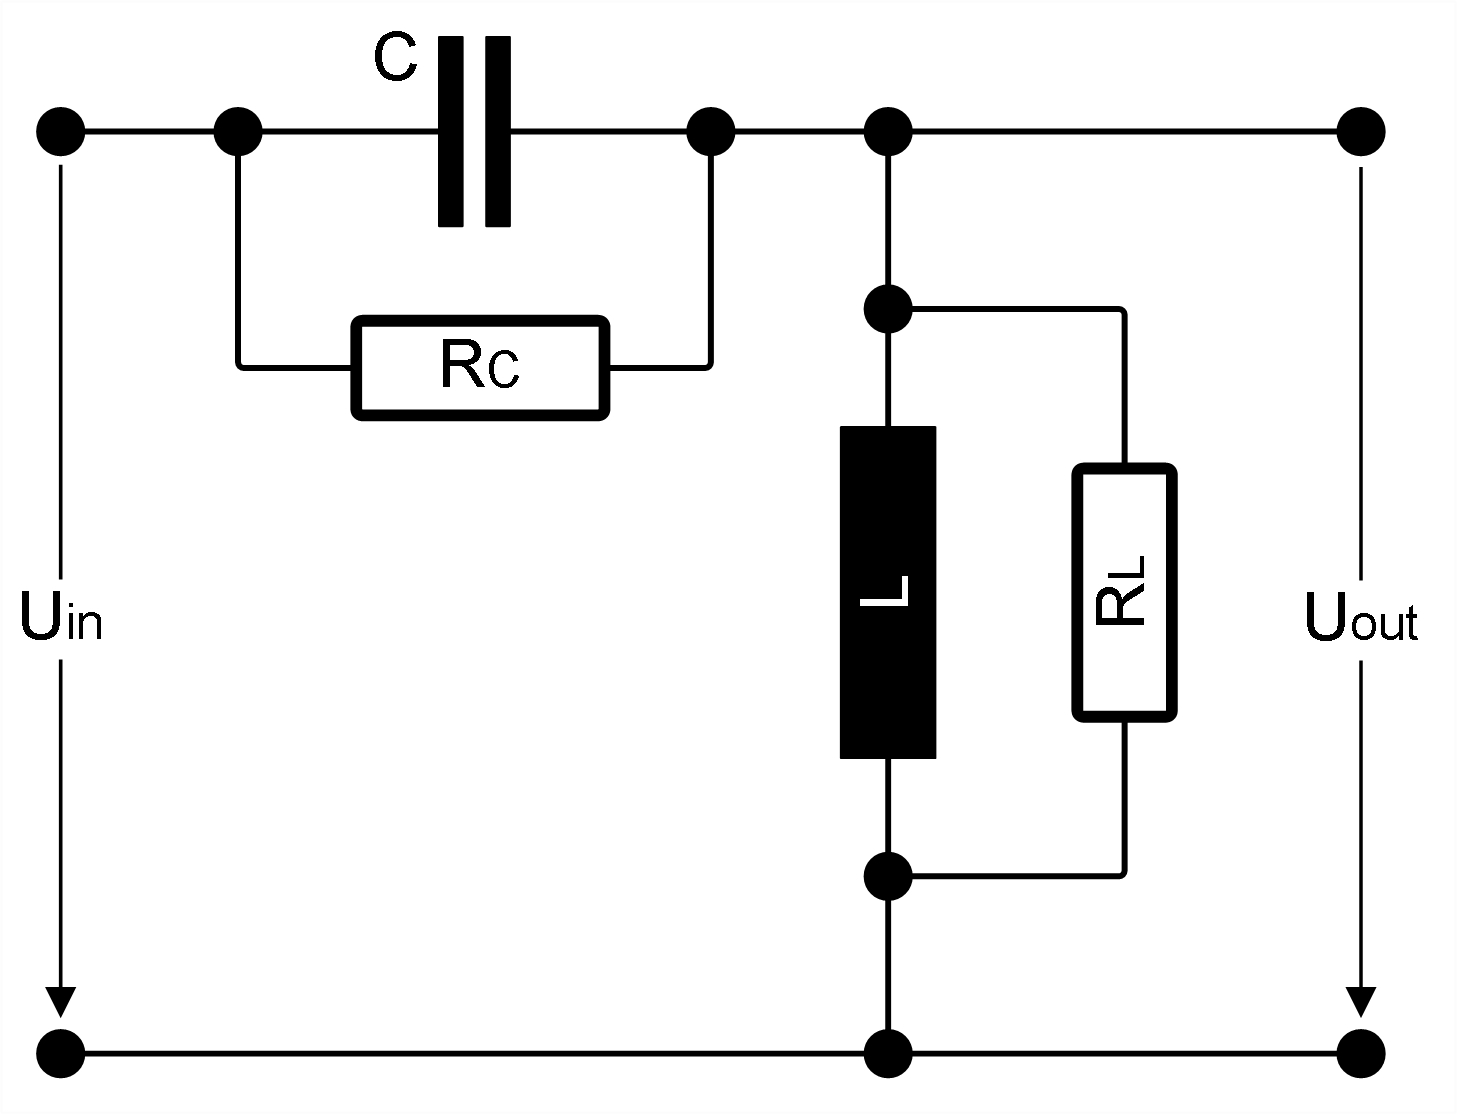
\includegraphics[width=5.06cm]{Impedance}
\\

\end{tabular}
\caption{RLC circuit}
\label{figImpedance}
\end{center}
\end{figure}
} % End of sample circuit: RLC circuit to demonstrate I/O impedance computation


The focus of this use case is put on the definition of the results. The
circuit itself is a simple damped LC resonator.

The user-defined result \ident{G} is the conventional transfer function
from stimulating input voltage $U_{in}$ to resulting output voltage
$U_{out}$. We have already seen this in a previous use case.

The definition of result \ident{Zin} is new. Line \verb+PLOT Zin Uin I_Uin+
requests the transfer function that expresses the dependency of the input
voltage on the input current. The ratio of these two is the input
impedance and we will get it as a function of the signal frequency~$s$. This
function will contain the static DC input impedance as limit $s \to 0$. The
new aspect of this result definition is that the dependent quantity, the
input voltage $U_{in}$, actually is a known quantity to the internal
computation; it's the device constant of the constant voltage source,
which provides the stimulating input voltage. Vice versa, the independent
quantity of the result, the input current $I_{U_{in}}$, is an unknown to the
internal computation. With respect to the internal computation result
\ident{Zin} is the request for an inverse transfer function. \linnet{}
supports inverse transfer functions with the following limitations:
\begin{itemize}
  \item Inverse transfer functions are limited to pairs of two quantities.
    There's no concept of an inverse full result
  \item In MIMO systems one and only one of the two quantities needs to be
    an independent quantity to the internal computation. Or with other
    words: one of the two quantities is a system input
\end{itemize}
The last constraint causes an inconvenience. Usually and like in figure
\ref{figImpedance} the input voltage is connected to a particular node $N$
and the ground node. In which case the voltage potential of node $N$ will
be identical to the input voltage; but regardless of the triviality of
this result it is a dependent quantity to the internal computation. If the
impedance is defined as the dependency of node $N$'s voltage potential on
the input current then this result definition will be invalid for a MIMO
system. As it is natural to name this particular node \code{in} and since
the unknown node potential is addressed to by prefixing this name with
\code{U\_} it becomes a matter of \code{Uin} or \code{U\_in} whether the
result definition is valid or invalid, respectively.

The constraint disappears for SIMO systems: If the system only has a
single input then the relationship between two dependent quantities is well
defined; both follow a modulation of the only input in a certain,
computable way and hence their relationship is known.

In principle, this behavior is natural and easy to understand but it might
be hard to accept due to the in practice typically very similar names of a
voltage source's device constant and the connected node's voltage
potential.

For our example \linnet{} returns:
\begin{verbatim}
RESULT - User-defined result Zin (Bode plot):
The dependency of Uin on I_Uin:
  Uin(s) = N_Uin_I_Uin(s)/D_Uin_I_Uin(s) * I_Uin(s), with
    N_Uin_I_Uin(s) = Rc*Rl*L*C * s^2
                     +(Rc*L + Rl*L) * s
                     +Rc*Rl
    D_Uin_I_Uin(s) = Rc*L*C * s^2
                     +(Rc*Rl*C + L) * s
                     +Rl
\end{verbatim}
The input impedance is the transfer function
\code{N\_Uin\_I\_Uin(s)/D\_Uin\_I\_Uin(s)}. The limit of this function for
$s \to 0$ is $R_C$. For DC operation the capacitor is as not present and
the impedance short-circuits the resistor $R_L$. The remaining resistance
from the input side is $R_C$.

The limit $s \to \infty$ can also be interpreted. The formula yields $R_L$
in this case. For very high frequencies the capacitor short-circuits the
resistor $R_C$ and $L$'s impedance goes against $\infty$. The parallel
resistor $R_L$ is the remaining resistance from the input side.

Between these two ends the magnitude of the complex function has a local
minimum.

If we run the generated Octave script \file{Zin.m} to plot the input
impedance then the standard Bode plot settings are used. Which means that
the $y$ axis is scaled in decibel. For the purpose of an impedance value
maybe not the most convenient convention. To get the values in Ohm
you will have to inverse the dB definition, if you e.g. read a value of
80\,dB in the plot then type \verb+10^(80/20)+ on the Ocatve command
line to get the impedance in Ohm.

Alternatively you can evaluate the generated transfer function for a given
frequency $f$ in Hz. In Octave this is as simple as typing
\code{abs(Zin()(2*pi*f))}.\footnote{In MATLAB the LTI transfer function
objects behave differently; the sample code won't work. You may instead
use function \ident{bode} with parameter $\omega=2 \pi f$ to get the
impedance value at frequency $f$.}

The computation of the output impedance is not that straightforward. It is
defined as the ratio of the output voltage drop caused by an output
current and this current. To put this in \linnet{} manageable terms we
need to extend the circuit by a load. If we use a current source then the
output impedance is the dependency of the output voltage on this load
current. The netlist in figure \ref{figImpedance} already contains a load
current source, see line \verb+I Iload gnd K2+. (Insofar the schematic on
the right hand side of the figure doesn't represent the circuit actually
computed by \linnet{}.)

We define the load current influent to the circuit. A negative voltage
change (a voltage drop) will be caused by a negative current and the
demanded ratio of both will become positive; this is the conventional sign
definition for an output impedance.

Please note, that the extension of the circuit doesn't necessarily need to
be done in a separate step. Other user-defined \code{PLOT} results, e.g.
the transfer function $G$, do not suffer from this additional current
source. If we demanded the full result for the output voltage then we'd
get a changed formula, now with two addends instead of a single term: Each
describing the impact of one of the sources on the output voltage. The
partial transfer function $G$ is just one of these two addends and doesn't
depend on the load current.

The rest holds as for the input impedance. The definition of the output
impedance $Z_{out}$ as \linnet{} result is made in line
\verb+PLOT Zout Uout Iload+. After running \linnet{} you will discuss the found formula:
\begin{verbatim}
RESULT - User-defined result Zout (Bode plot):
The dependency of Uout on Iload:
  Uout(s) = N_Uout_Iload(s)/D_Uout_Iload(s) * Iload(s), with
    N_Uout_Iload(s) = Rc*Rl*L * s
    D_Uout_Iload(s) = Rc*Rl*L*C * s^2
                      +(Rc*L + Rl*L) * s
                      +Rc*Rl
\end{verbatim}
or run the generated Octave script \file{Zout.m} to plot the impedance or
compute its values at particular frequencies. The Octave computations can
be done for particular device values only; these are not configured in
our example netlist and Octave will begin with initial standard values.


\section{Transistor model}

The final use case is the complexest one. Figure \ref{figBipolarTModel}
shows a typical transistor amplifier circuit. The input voltage $U_{in}$
is amplified to the output voltage $U_{out}$. Main characteristics of the
circuit is the frequency response of the output in dependency of the
input. This uses case demonstrates the usage of \linnet{} in the analysis
of such a prototypical circuit.

% Sample circuit: Model of inverting op-amp.
{
% This define is related to the specifics of the array package; see
% http://texwelt.de/wissen/fragen/3401/zentrieren-text-in-tabelle (as of
% July 25 2014) for more
\newcolumntype{M}[1]{>{\centering\arraybackslash}m{#1}}

\begin{figure}
\begin{center}
\begin{tabular}{M{7cm}M{8.3cm}}
{\normalsize
\verbatiminput{BipolarTModel.cnl}
}
&
% The ideal width of the figure to get the same scale of the device as in
% the other schematics would be 8.51cm. This leads to a total width of the
% figure greater than \textwidth. Having a somewhat smaller scale seems to
% be the better choice in this case.
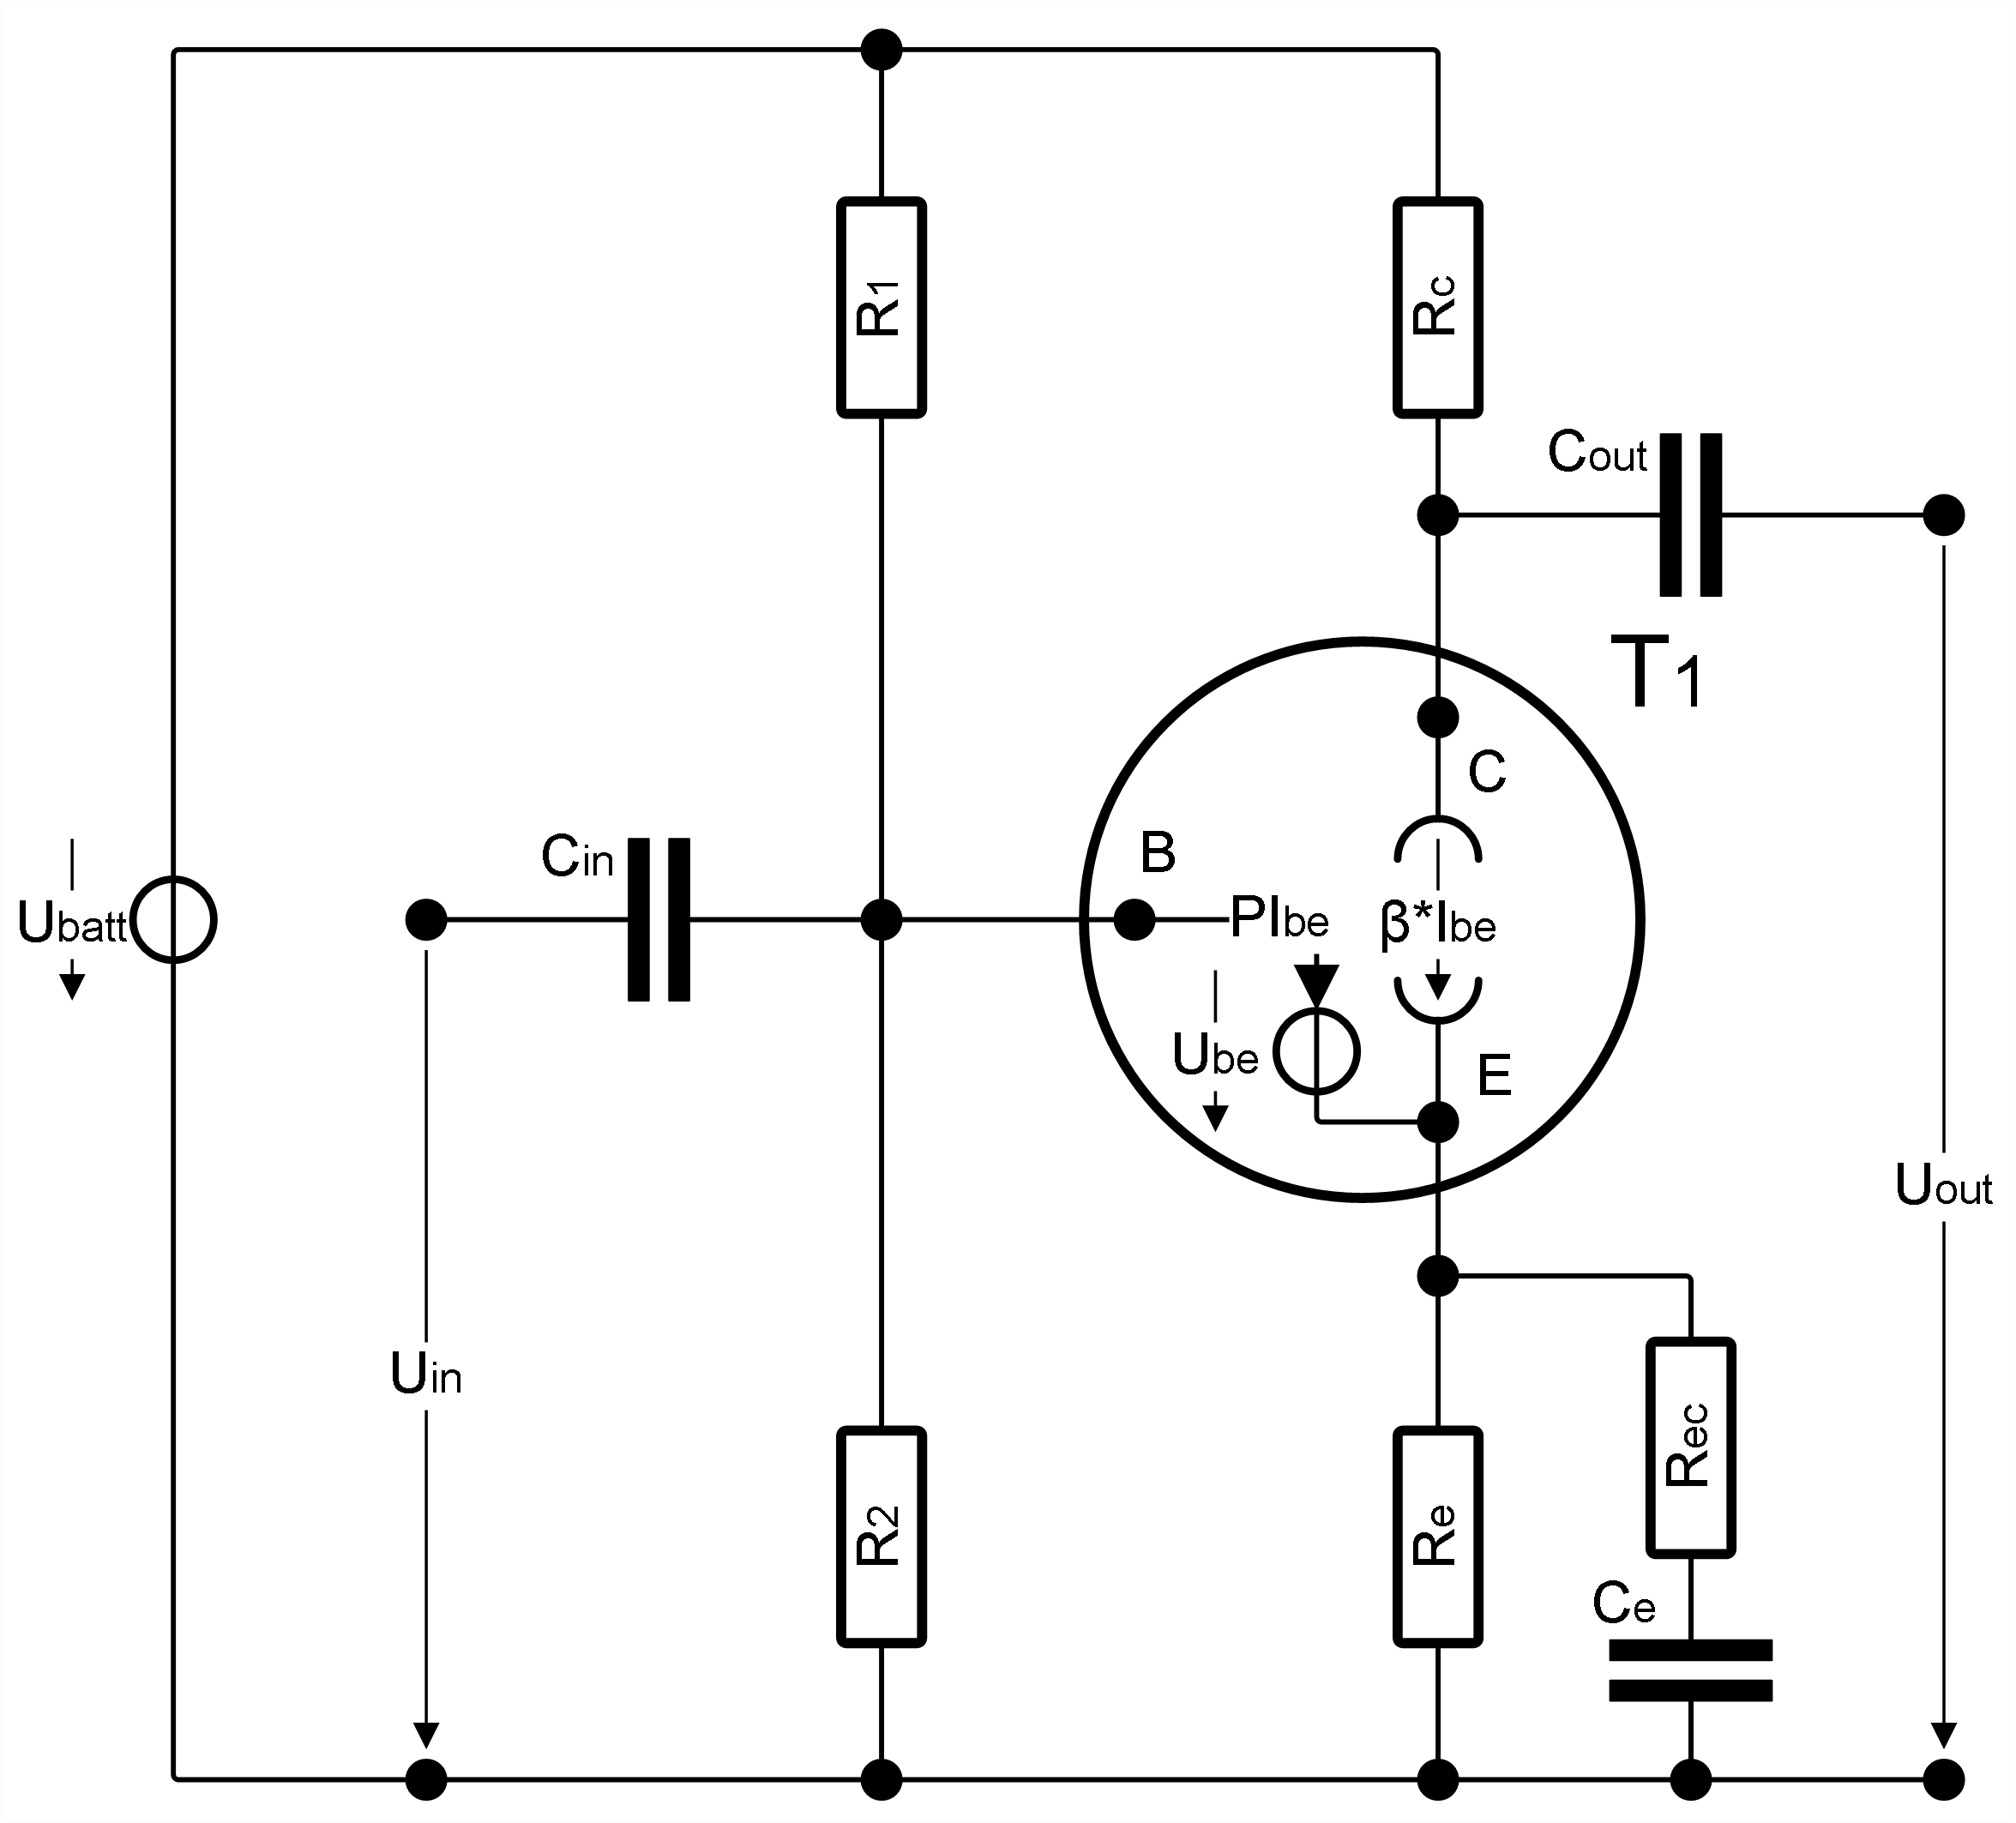
\includegraphics[width=8.3cm]{BipolarTModel}
\\

\end{tabular}
\caption{Bipolar transistor amplifier}
\label{figBipolarTModel}
\end{center}
\end{figure}
} % End of sample circuit: Model of inverting bipolar transistor amplifier.


\subsection{Circuit design}

Initially, a rough calculation is made that leads to an initial set of
numeric device values. The results of the later \linnet{} computation can
then be used to prove the made simplifications and to validate and perhaps
refine the initial findings.

The design of the circuit is driven by some requirements and figured out
based on some simplifications. Let's assume the following requirements:
\begin{itemize}
  \item The amplification should be about 100 or 40\,dB
  \item The output impedance should be in the magnitude of 10\,k$\Omega$
  \item The amplifier should be operational in a frequency range of
    100\,Hz \dots 20\,kHz
  \item The circuit should have a stable operating point
\end{itemize}

The starting point of the design is the yielded amplification. The nominal
current amplification $\beta$ of our transistor be 250. This leaves room
for an emitter current based feedback: The rising voltage at the emitter
resistor due to current amplification will be a counter-control of the
amplification as it directly decreases the base-emitter voltage
drop.\footnote{In the true implementation of the circuit such a feedback
reduces the impact of the non linearity of the real transistor device.
This can't be illustrated, proven or quantified with \linnet{} as
\linnet{} can't model any kind of nonlinearity.}

The emitter voltage nearly follows the input voltage and the current
through the emitter is nearly the current through the collector;
consequently, the expected amplification (disregarding the inversion) is
about the ratio of collector to emitter resistor,
$\left| V \right| \simeq R_c/R_{e_{eff}}$.

A further simplification is that the collector current is relatively
independent of the circuitry in the collector. An hypothetical output
current will therefore always mean an additional voltage drop at $R_c$,
which is proportional to this resistor and the hypothetical current. This
means that the circuit's output impedance has nearly the same value as
$R_c$. According to our requirement we choose a value of $R_c=6.8$\,k, which
means $R_{e_{eff}} \simeq 68\,\Omega$.

The operating point of the collector (i.e. the voltage at input voltage
null) should be somewhat above the middle of the supply voltage to get a
symmetric limit for both polarities of the input voltage. Given $R_c=6.8$\,k
we want to have a collector current
$I_c=5.7\text{\,V}/6.8\text{\,k}\Omega=0.84\text{\,mA}$. It holds
$I_c \simeq I_e$ and accordingly $U_b \simeq U_{be} + R_{e_{eff}} I_c$.
The actual base voltage will be set with the ratio $R_1/R_2$. As $U_{be}$
is considered constant the product $R_{e_{eff}} I_c$ will have to
compensate for any deviation of $U_b$ from the targeted value due to
tolerances of $R_1$ or $R_2$. The larger $R_{e_{eff}}$ the smaller the
deviation of $I_c$ and thus of the targeted operating point.
This consideration explains the emitter circuitry: For DC currents we want
to have a large value to get a stable and targeted operating point but the
design goal $V=100$ already demanded a value of 68\,$\Omega$ for the
relevant input frequency range. The answer is: Place the 68\,$\Omega$ behind
a DC blocking capacitor and put a larger resistor for DC operation in
parallel. We take the tenfold value for DC operation, $R_e=680\,\Omega$;
this won't affect the previous findings too much or with other words,
$R_{e_{eff}}$ for the relevant input frequency range. For DC operation the
effective emitter resistance is $R_e$ and the wanted value for $U_b$ becomes 
$U_b=0.6\text{\,V}+680\text{\,}\Omega \cdot 0.84\text{\,mA}=1.17\text{\,V}$.

The last step of the design is the voltage divider at the transistor's
base. The simplification used here is that the base current can be
neglected in comparison to the currents through the two resistors. This
leads to the simple formula $U_b = R_2/(R_1+R_2) U_{batt}$. Considering
only resistor values from the E12 series (10\% tolerance) we choose 10\,k
and 1.2\,k to get the best fit. The current through the resistors is about
one Milli Ampere, which is a hundredfold of the base current $I_c/\beta$ so
that the made simplification is applicable.


\subsection{Modelling the transistor circuit}
 
Normally a circuit like this is modeled as a so called small-signal
circuit. The true circuit is reduced to those elements, which are relevant
for the frequency response above $f=0$. The resulting circuit would no
longer be operational in a true construction and the DC operating point
can't be computed any longer. In a second step one would then do the
contrary to figure out the DC behavior. Using \linnet{} we can decide to
model all at once.

To \linnet{} the circuit is a system with three independent inputs and a
list of dependent quantities under which our output voltage $U_{out}$. For
us, the two inputs $U_{batt}$ and $U_{be}$ are constant values, we will
have to put the constant values 12\,V and 0.6\,V into the resulting
formulas. However, seeing $U_{batt}$ as a true input signal we can easily
find e.g. the hum suppression of the circuit: Consider $U_{batt}$ had a
frequency component of the public power grid and ask for the transfer
function from power supply to output voltage.

\subsubsection{The transistor model}

The bipolar NPN transistor itself is modeled as an ideal current
amplifier; the collector current is assumed to be $\beta$ times the base
current, where $\beta$ is a constant. It is modeled without
non-linearities and frequency dependencies. To get a full picture of the
DC behaviour the voltage drop from base to emitter is modeled by a
constant voltage source of 0.6\,V.

The current amplification is implemented by a current controlled current
source. The device constant is the factor between the source's current and
the control current. Obviously, the former is the collector current and
the latter the base current. \linnet{} takes a device's name as device
constant in the result representation. Therefore we name the device
\ident{beta}.

The current controlled current source references a current probe to
specify the control current. The probe is placed in series to the base of
the transistor and senses the base current. The name of the probe is
\ident{I\_base} and \linnet{} will use the same name for the sensed
current if it should be referenced from a result definition. (If the
probe's name wouldn't begin with \code{I\_} then \linnet{} would add this
as a prefix in order to make transparent that the referenced quantity is a
current.)


\subsection{The voltage amplification}

The principal characteristics of the transistor circuit is the resulting
amplification, the ratio of magnitudes of out- and input voltage. Due to
the decoupling capacitors we have amplification null for DC. We have to
define the amplification as the voltage ratio at frequencies above the
influence of the capacitors.

We look at the partial result for the output voltage, which only describes
its dependency on the input voltage.

\begin{verbatim}
RESULT - User-defined result G (Bode plot):
The dependency of U_out on Uin:
  U_out(s) = N_U_out_Uin(s)/D_U_out_Uin(s) * Uin(s), with
    N_U_out_Uin(s) = -(beta*R1*R2*Rc*Re*Ce*Cin + beta*R1*R2*Rc*Rec*Ce*Cin) * s^2
                     -beta*R1*R2*Rc*Cin * s
    D_U_out_Uin(s) = (beta*R1*R2*Re*Rec*Ce*Cin + R1*R2*Re*Rec*Ce*Cin) * s^2
                     +(beta*R1*R2*Re*Cin + beta*R1*Re*Rec*Ce + beta*R2*Re*Rec*Ce
                       + R1*R2*Re*Ce + R1*R2*Re*Cin + R1*R2*Rec*Ce + R1*Re*Rec*Ce
                       + R2*Re*Rec*Ce
                      ) * s
                     +(beta*R1*Re + beta*R2*Re + R1*R2 + R1*Re + R2*Re)
\end{verbatim}

Due to our initial considerations we take this result for high input
frequencies, i.e. for high frequencies of $U_{in}$. The amplification $V$
is got as limit $s \to \inf$. We take the quotient of the numerator and
denominator terms of highest power in s:

\begin{eqnarray}
V & = & \lim_{s \to \inf}G(s)
        = - \frac{\beta R_1 R_2 R_c R_e C_e C_{in} + \beta R_1 R_2 R_c R_{ec} C_e C_{in}}
                 {\beta R_1 R_2 R_e R_{ec} C_e C_{in} + R_1 R_2 R_e R_{ec} C_e C_{in}}
        = - \frac{\beta R_c R_e + \beta R_c R_{ec}}{\beta R_e R_{ec} + R_e R_{ec}}
\nonumber \\
  & = & - \frac{\beta}{\beta+1} \frac{R_c}{\frac{R_e R_{ec}}{R_e+R_{ec}}}
\label{eqTAmplification}
\end{eqnarray}

The result (\ref{eqTAmplification}) for the amplification can be
interpreted. $V$ is mainly determined by the second term, which can be
read as the ratio of collector resistor to the parallel circuit of the two
emitter resistors; the emitter capacitor behaves as if not present for
high frequencies.

The earlier made approximation of $V$ as the ratio of the collector
resistor's value and the effective resistance at the emitter was based on
the idea that the same current flew through both resistors and leads to
voltage magnitudes proportional to their values, while due to the constant
$U_{be}$ the voltage drop at the emitter resistor follows the input
voltage. Now we get the corrective first term in
equation~(\ref{eqTAmplification}), which is a number closed to one and
reduces the approximation of the amplification a tiny bit. It expresses
that the currents through emitter and collector are indeed similar but not
identical. The voltage modulation at the collector has to be reduced by
the portion of the base current.

% The content of the next section is double. The same consideration can
% be found in section {In- and output impedance of a circuit}, behind the
% enumeration of the MIMO constraints.
%
% \subsubsection{Important note: Addressing to independent quantities in
% MIMO systems}
% 
% At this point a quite specific and maybe hard to accept behavior of
% \linnet{} will be explained.
% 
% The user-defined Bode result \ident{G} has been requested by the valid
% line
% 
% \verb+PLOT G U_out Uin  LOG 50 10 20k+
% 
% \noindent in the input file. The definition means that voltage potential
% \ident{U\_out} is plotted in dependency of voltage \ident{Uin}. For this
% plot, \ident{Uin} is the independent quantity and \ident{U\_out} the
% dependent quantity. \ident{Uin} refers to the device constant of the
% driving voltage source, which is a known, independent quantity to the
% internal computation.
% 
% The voltage source is connected to nodes \ident{in} and \ident{gnd}. The
% voltage potential of node \ident{in} will become a variable of the
% internal computation. The name of this variable (as explained above) is
% known to be \ident{U\_in}. Since the second connector of the source is the
% ground node it's evident that the voltage potential of this node will be
% identical to the source's constant voltage. The alternative, nearly
% identical line
% 
% \verb+PLOT G U_out U_in  LOG 50 10 20k+
% 
% \noindent
% will however fail to produce a result. To the internal computation
% \ident{U\_in}, the node \ident{in}'s voltage potential, is an unknown,
% dependent quantity -- different to the given source's voltage \ident{Uin}.
% And for MIMO systems it is generally forbidden to request a Bode plot
% where two dependent quantities (with respect to the internal computation)
% depend on each other. If a system has more than a single input than the
% relationship of two dependent quantities is not defined; in general it'll
% differ depending on the input, which is modulated.
% 
% In principle, this behavior is natural and easy to understand but it might
% be hard to accept due to the in practice typically very similar names of a
% voltage source's device constant and the connected node's voltage
% potential.


\subsection{Limits of operational range of transistor}
\label{secTModelOpLimits}

The limitations of the true transistor can't be considered by \linnet{}
(as any non-linearity) and nothing about can be seen in any of the
results.

\begin{figure}
  \centering
  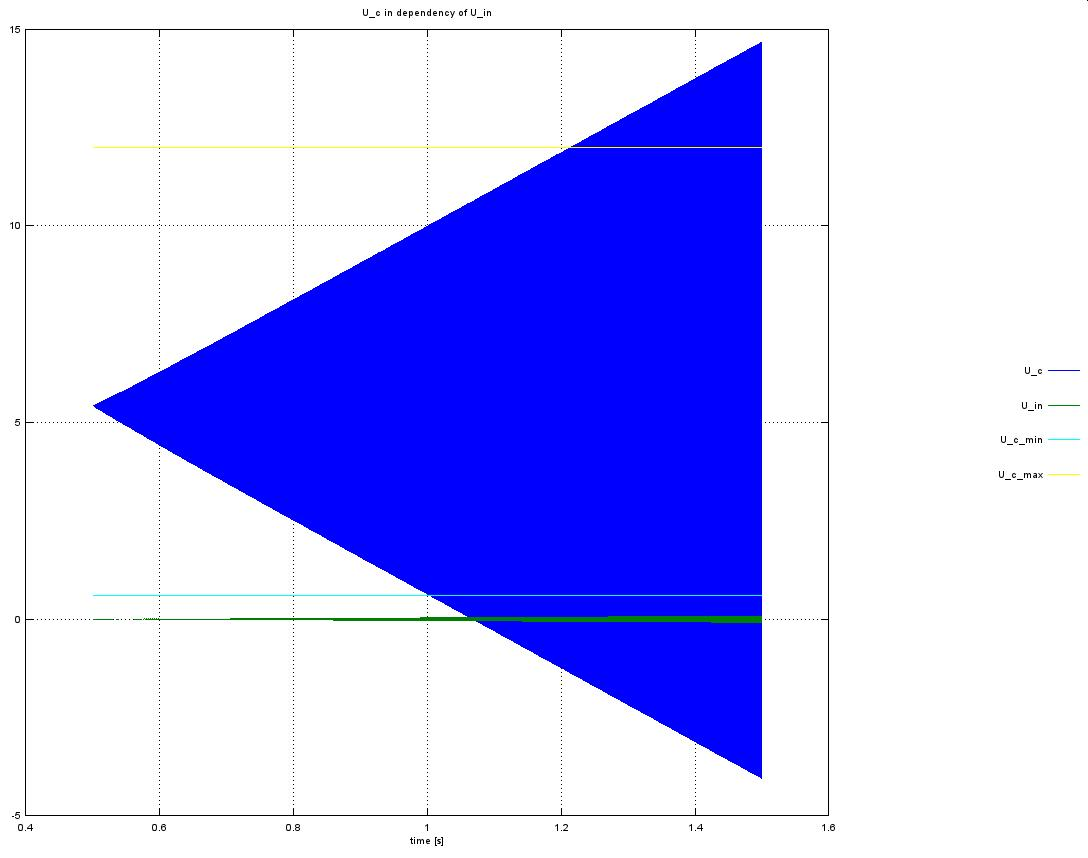
\includegraphics[width=0.7\textwidth]{BipolarTModel_lsim}
  \caption{Simulation of bipolar amplifier circuit in figure
    \ref{figBipolarTModel} with modulated sinoid input
  }
  \label{figBipolarTModel_lsim}
\end{figure}


As an idea to investigate the limits of the amplification we could request
the result for the voltage $U_c$. The true ciruit reaches its limits if
this voltage approaches either $U_{batt}$ or $U_e$ ($U_e$ is nearly
constant by design). In the numeric post-processing with Octave we could
plot this quantity for a rising input signal and compare $U_c$ with
these limits. The point in time, when it first reaches one of the limits
designates the maximum in- and output signal, which could be processed by
a real implementation of the simulated circuit.

This is in one respect a new technique. So far, we focussed on transfer
functions from one quantity to another one. For this investigation we need
to simulate all the inputs since the DC operating point is an essential
part of this computation. Neither the frequency response analysis nor the
step response analysis Ocatve offers will suffice. We need to do a time
domain simulation using all the inputs simultaneously.

An Octave script assembles the required input signal as a 3-column vector
of samples and creates the LTI system object using the \linnet{} generated
result script. Then it runs this system with the input signal. The
simulation result for $U_c$ is shown in figure
\ref{figBipolarTModel_lsim}. At $t=1$\,s the lower limit for $U_c$ is
reached. At this time the input signal has an amplitude of 50\,mV. This is
the maximum input value the true circuit could process without truncation.
The figure shows that the operating point is not yet optimal; both limits
should be reached at the same time to optimally exploit the available
operating range.

The Octave script is printed as listing \ref{lstSimBipolarTModel} on page 
\pageref{secListingOctaveSimulation}. Please refer to this listing to
get more details on how to run a \linnet{} generated LTI system with
arbitrary input signals.

Using a former result, the amplification $V$, another approach is possible.
If we achieved the design goal that the operating point for the collector is
in the center of the possible output voltage range then we can compute the
maximum undistorted peak-peak input voltage by dividing this range by
the found amplification. The found result should nearly be the same as
with the time domain simulation and it would be formula based.

The design goal ``operating point for collector voltage'' can be validated by
demanding the full result for $U_c$ and evaluating the formula for
$U_{in}(s)=0$ and $s=0$. \linnet{} reports for $U_c$:
\begin{verbatim}
RESULT - User-defined result DC:
The solution for unknown U_c:
  U_c(s) = N_U_c_Ubatt(s)/D_U_c_Ubatt(s) * Ubatt(s)
           + N_U_c_Uin(s)/D_U_c_Uin(s) * Uin(s)
           + N_U_c_Ube(s)/D_U_c_Ube(s) * Ube(s), with
    N_U_c_Ubatt(s) = (beta*R1*R2*Re*Rec*Ce*Cin + R1*R2*Re*Rec*Ce*Cin) * s^2
                     +(beta*R1*R2*Re*Cin + beta*R1*Re*Rec*Ce - beta*R2*Rc*Re*Ce
                       - beta*R2*Rc*Rec*Ce + beta*R2*Re*Rec*Ce + R1*R2*Re*Ce
                       + R1*R2*Re*Cin + R1*R2*Rec*Ce + R1*Re*Rec*Ce + R2*Re*Rec*Ce
                      ) * s
                     +(beta*R1*Re - beta*R2*Rc + beta*R2*Re + R1*R2 + R1*Re
                       + R2*Re
                      )
    D_U_c_Ubatt(s) = (beta*R1*R2*Re*Rec*Ce*Cin + R1*R2*Re*Rec*Ce*Cin) * s^2
                     +(beta*R1*R2*Re*Cin + beta*R1*Re*Rec*Ce + beta*R2*Re*Rec*Ce
                       + R1*R2*Re*Ce + R1*R2*Re*Cin + R1*R2*Rec*Ce + R1*Re*Rec*Ce
                       + R2*Re*Rec*Ce
                      ) * s
                     +(beta*R1*Re + beta*R2*Re + R1*R2 + R1*Re + R2*Re)
    N_U_c_Uin(s) = -(beta*R1*R2*Rc*Re*Ce*Cin + beta*R1*R2*Rc*Rec*Ce*Cin) * s^2
                   -beta*R1*R2*Rc*Cin * s
    D_U_c_Uin(s) = D_U_c_Ubatt(s)
    N_U_c_Ube(s) = (beta*R1*R2*Rc*Re*Ce*Cin + beta*R1*R2*Rc*Rec*Ce*Cin) * s^2
                   +(beta*R1*R2*Rc*Cin + beta*R1*Rc*Re*Ce + beta*R1*Rc*Rec*Ce
                     + beta*R2*Rc*Re*Ce + beta*R2*Rc*Rec*Ce
                    ) * s
                   +(beta*R1*Rc + beta*R2*Rc)
    D_U_c_Ube(s) = D_U_c_Ubatt(s)
\end{verbatim}

The operating point for $U_c$ is found as:
\begin{eqnarray}
U_{C0} & = & \frac{(\beta R_1 R_e - \beta R_2 R_c + \beta R_2 R_e + R_1 R_2 + R_1 R_e
                    + R_2 R_e
                   ) U_{batt}
                   + (\beta R_1 R_c + \beta R_2 R_c) U_{be}
                  }
                  {\beta R_1 R_e + \beta R_2 R_e + R_1 R_2 + R_1 R_e + R_2 R_e}
\nonumber \\
       & = & U_{batt} - \frac{\beta R_c}{R_1 R_2 + (1+\beta) (R_1+R_2) R_e}
                        [R_2 U_{batt} - (R_1+R_2) U_{be}]
\label{eqTOperatingPoint}
\end{eqnarray}

Copying the formula (\ref{eqTOperatingPoint}) into Octave and using
$U_{be}=0.6$\,V and $U_{batt}=12$\,V we get $U_{c0}=5.21$\,V.
This is not optimal; taking the constant emitter voltage of about 0.6\,V
into account the ideal value would be about 1\,V higher; a refinement of
the device values can be suggested.

Using Octave we can find out on the fly that the dependency of the
operating point on the transistor amplification $\beta$ is negligible; the
variation $\beta=150 \ldots 300$ yields a variation $U_{c0}=5.26\text{\,V} \ldots
5.20\text{\,V}$.\footnote{The fasted way to reproduce these values is to directly
use the \linnet{} generated LTI object to evaluate the transfer function
at s=0 and to compute the output as linear combination of the three input
contributions:
\verb~
[sys p]=DC;
p.beta=150, sys=DC(p),
F0=sys(0), U\_c0=F0(1,:)*[12; 0; 0.6]~
The first statement is only used to get parameter object \ident{p} that
can then be manipulated for the variation of $\beta$.}
This is important insofar as the transistor amplification has a
high standard deviation for a given device type. A more profound
investigation could even state this as a formula, we can easily figure
out the partial derivative of (\ref{eqTOperatingPoint}) with respect to
$\beta$.

Another aspect: The partial derivatives of (\ref{eqTOperatingPoint}) with
respect to $\beta$ and the resistors would prove whether the trick with
$C_e$ and $R_{ec}$ in parallel circuit to $R_e$ really pays off: it has
been made to reach the design goal for the amplification $V$ without
endangering a stable operating point. If the operating point would however
still be tolerant against typical standard deviations of $\beta$ and the
resistors for a ten times smaller value of $R_e$ then we could live
without this trick.


\subsection{Hum suppression}

The hum suppression might be of interest for a real application of the
circuit if it has a conventional power supply, which might contain some
remains of the 50\,Hz frequency of the public grid. Hum suppression
describes to which extend such remains will be apparent at the circuit
output.

The dependency of the collector voltage $U_c$ on the supply voltage
$U_{batt}$ is part of the user-defined result \ident{DC}, which we had
discussed in the previous section. Even more convenient than evaluating result
\ident{DC} is to specify a result, which is more to the point. Please,
refer to line

\verb+PLOT humSupp U_out Ubatt  LOG 500 10 100+

in the circuit netlist: We demand the dedicated result \ident{humSupp} and
will get an Octave script of same name. The computed formula is exactly
the extract of the full result \ident{DC}, which we need. The default
behavior of the Octave script \file{humSupp.m }is to present the result as
a Bode plot. All we have to do is to run the script and to read the plot
at the frequency of the public power grid. We get a value of only
-0.3\,dB, which means that the hum is propagated to the circuit output
without noticeable damping.

The explanation: In the computation of a MIMO system and if we ask for the
transfer function of one of its inputs to one of its outputs, then the
answer holds under the assumption that the other inputs have given values,
e.g. null all the time (however the actual input function is irrelevant).
With other words its assumed that the inputs are driven with a source of
output impedance null. For our circuit this has the consequence that the
input capacitor $C_{in}$ stabilizes the base voltage of the transistor -
here we have a good hum suppression. Accordingly, the collector current is
also stablized but unfortunately this means that the collector voltage
exactely follows the battery voltage -- and this is what we read from the
Bode plot.

Please note that $C_{out}$ doesn't appear in the transfer function
$U_{batt}$ to $U_{out}$. All computation is ideal and since there's no
load the output capacitor is currentless all time long and hence has no
impact on the output voltage. In any true application of the circuit it
would introduce in conjunction with the input impedance of the following
stage a further time constant in the overall system behavior.


\subsection{Output impedance}

As seen in a previous use case the output impedance of the circuit can be
found by adding a defined load and asking for the dependency of the output
voltage on this load. If we add the lines
\begin{verbatim}
I    Iload gnd   out   
PLOT Zout  U_out Iload LOG 50 10 20k
\end{verbatim}
to the input file then \linnet{} finds a formula of third order in $s$ for
the output impedance. The limit of its value for $s \to 0$ is infinite.
This is expected as the capacitor $C_{out}$ decouples the DC component
from the output signal. The limit for $s \to \infty$ is identical to $R_c$
and in the Bode plot we see that this final value is reached at about
100\,Hz, thus at the beginning of our defined frequency operation range.
This meets our initial expectations.

The picture becomes even clearer if we modify the additional lines in the
input file like this:
\begin{verbatim}
I    Iload gnd c
PLOT Zout  U_c Iload LOG 50 10 20k
\end{verbatim}
Using these lines we actually remove the decoupling output capacitor from
the circuit and define the output impedance at the collector of the
transistor. Now \linnet{} computes the resulting transfer function as:
\begin{verbatim}
RESULT - User-defined result Zout (Bode plot):
The dependency of U_c on Iload:
  U_c(s) = N_U_c_Iload(s)/D_U_c_Iload(s) * Iload(s), with
    N_U_c_Iload(s) = Rc
    D_U_c_Iload(s) = 1
\end{verbatim}
The proportionality factor between current and voltage is identical to the
value $R_c$ of the collector resistor -- this is what we had assumed in
our initial design simplifications.
